\section{Концентрация меры}
\subsection{Введение}



Число $\mu _f $ называют медианой функции $f$, если
\begin{equation*}
\mu \left( {\vec {x}\in S_1^n :\;\;f\left( {\vec {x}} \right)\ge \mu _f } 
\right)\ge 1 \mathord{\left/ {\vphantom {1 2}} \right. 
\kern-\nulldelimiterspace} 2
\quad \text{и} \quad 
\mu \left( {\vec {x}\in S_1^n :\;\;f\left( 
{\vec {x}} \right)\le \mu _f } \right)\ge 1 \mathord{\left/ {\vphantom {1 
2}} \right. \kern-\nulldelimiterspace} 2,
\end{equation*}

где $\mu \left( {d\vec {x}} \right)$ - равномерная мера на единичной сфере 
$S_1^n $ в ${\rm R}^n$. Пусть $A$ - измеримое (борелевское) множество на 
сфере $S_1^n $. Через $A_\delta $ - будем обозначать $\delta $-окрестность 
множества $A$ на сфере $S_1^n $.  Оказывается, что если $\mu \left( A \right)\ge 1 \mathord{\left/ 
{\vphantom {1 2}} \right. \kern-\nulldelimiterspace} 2$, то
\[
\mu \left( {A_\delta } \right)\ge 1-\sqrt {\pi \mathord{\left/ {\vphantom 
{\pi 2}} \right. \kern-\nulldelimiterspace} 2} \exp \left( {-{\delta ^2n} 
\mathord{\left/ {\vphantom {{\delta ^2n} 2}} \right. 
\kern-\nulldelimiterspace} 2} \right).
\]

Иллюстрацией этому результату является задача о царице Дидоне: царь предложил царице построить 
огород с заданной длиной забора,а царица хочет, чтобы её участок земли при заданном 
периметре имел наибольшую площадь. Таким образом, царице надо решить 
изопериметрическую задачу (такие задачи обычно рассматриваются в курсах 
вариационного исчисления). Решение этой задачи хорошо известно -- <<круглый 
огород>>. Рассмотрение двойственной задачи (при заданной площади огорода, минимизировать его периметр) приводит к результату для $\mu(A_{\delta})$. 


Пусть теперь на $S_1^n $ задана функция с модулем непрерывности
\[
\omega _f \left( \delta \right)=\sup \left\{ {\left| {f\left( {\vec {x}} 
\right)-f\left( {\vec {y}} \right)} \right|:\;\;\rho \left( {\vec {x},\vec 
{y}} \right)\le \delta ,\;\vec {x},\vec {y}\in S_1^n } \right\}.
\]
Тогда
\[
\mu \left( {\vec {x}\in S_1^n :\;\;\left| {f\left( {\vec {x}} \right)-\mu _f 
} \right|\ge \omega _f \left( \delta \right)} \right)\le \sqrt {\pi 
\mathord{\left/ {\vphantom {\pi 2}} \right. \kern-\nulldelimiterspace} 2} 
\exp \left( {-{\delta ^2n} \mathord{\left/ {\vphantom {{\delta ^2n} 2}} 
\right. \kern-\nulldelimiterspace} 2} \right).
\]




Можно показать, что при весьма естественных условиях медиана асимптотически 
близка к среднему значению (математическому ожиданию). Аналогичное 
неравенство можно получить (М. Талагран, 1994), например, для модели 
случайных графов (Эрдёша - Реньи). И исследовать плотную концентрацию около 
среднего значения различные функций на случайных графов: число 
независимости, хроматическое число и т.п..

\medskip
%\medskip
%\textbf{
%TODO Неравенство Талаграна 
%}
\medskip

Приведем неравенство Талаграна. Пусть заданы множества $\Sigma_i$, $i=1,\dots,n$, элементарных исходов. На этих множествах заданы вероятностные меры $P_i$, $i=1,\dots,n$. Положим 
\begin{equation*}
\Sigma = \prod_{i=1}^n\Sigma_i,\quad P = \prod_{i=1}^n P_i.
\end{equation*}
Введем взвешенную метрику Хэмминга:
\begin{equation*}
d_{\alpha}(x,y) = \sum_{x_i\not = y_i} \alpha_i \biggr/ \sqrt{\sum_{i=1}^n \alpha^2_i}
\end{equation*}
и определим $d_{\alpha}(x,A) = \min_{y\in A} d_{\alpha}(x,y)$, $\rho(x,A) = \sup_{\alpha\in \mathbb{R}^n} d_{\alpha}(x,A)$. Пусть $A\in \Sigma$. Определим $t$-окрестность ($t\geq$ 0) множества $A$ по формуле 
\begin{equation*}
A_t = \{x\in\Sigma: \rho (x,A)\leq t\}.
\end{equation*}
Тогда справедливо неравенство Талаграна:
\begin{equation*}
P(A)(1-P(A_t))\leq \exp\biggl(-\frac{t^2}{4}\biggr).
\end{equation*}

Интересным примером концентрации меры являются следующие результаты Вершика. 

\textbf{Предельные меры для задачи о распределении максимального цикла в подстановке и др.}
В качестве множества элементарных исходов рассматривается группа всевозможных 
подстановок (перестановок) $S_n $ (симметрическая группа), $n\gg 1$. В этой 
группе $n!$ элементов. Припишем каждой подстановке одинаковую вероятность $1 
\mathord{\left/ {\vphantom {1 {n!}}} \right. \kern-\nulldelimiterspace} 
{n!}$. Оказывается, что верны следующие результаты.
\begin{enumerate}
\item  Математическое ожидание числа циклов есть 
$\approx \ln n$.

\item  Нормированные длины циклов случайной 
подстановки убывают со скоростью геометрической прогрессии со знаменателем 
$e^{-1}$.

\item Положим $\rho _n \left( a \right)={\left| {\left\{ {g\in S_n 
:\;n_{\max } \left( g \right)\le an} \right\}} \right|} \mathord{\left/ 
{\vphantom {{\left| {\left\{ {g\in S_n :\;n_{\max } \left( g \right)\le an} 
\right\}} \right|} {n!}}} \right. \kern-\nulldelimiterspace} {n!}$, где 
$n_{\max } \left( g \right)$ - длина максимально цикла в подстановке $g$. 
Величина $\rho _n \left( a \right)$ удовлетворяет \textit{уравнению Дикмана -- Гончарова} (40-ые годы XX 
века):
$
\rho _n \left( a \right)=\int\limits_0^a {\rho _n \left( {\frac{a}{1-t}} 
\right)dt} .
$
\item  Начиная с некоторого большого числа $N$ 99{\%} 
натуральных чисел $n$, больших, чем $N$ обладают свойством
$
n^{0.99}<p_1 \cdot ...\cdot p_{11} ,
$
где $p_1,\dots, p_{11}$ наибольшие $11$ простых делителей при разложении числа на произведение простых чисел (среди $p_1,\dots,p_{11}$ может оказаться несколько одинаковых простых чисел).
Иначе говоря, у основной части (99{\%}) натуральных чисел основная часть 
(99{\%}) числа есть произведение наибольших простых делителей. Число 11 
возникло из-за того, что мы выбрали 99{\%} и 99{\%}.
\end{enumerate}

\medskip 

%Для доказательства неравенства Азумы необходимы следующие понятия и результаты.

% Пусть $\{Z_i\}^{n}_{i=1}$ и  $\{X_i\}^n_{i=1}$ последовательность случайных величин на одном вероятностном пространстве, таких что $\mathbf{E}[X_i|Z_1,\dots,Z_{i-1}] = X_{i-1}$ для всех $i$. Тогда $\{X_i\}^n_{i=1}$ называется мартингалом по отношению к $\{Z_i\}^{n}_{i=1}$. Более того последовательность $Y_i = X_i-X_{i-1}$ называется разностной мартингальной последовательностью. По определению  $\mathbf{E}[Y_i|Z_1,\dots,Z_{i-1}] = 0$ для всех $i$.
%Более общее определение: пусть $\{\mathcal{F}_i\}_{i=1}^n$ фильтрация, то есть вложенная последовательность $\sigma$-алгебр $\varnothing \subseteq \mathcal{F}_1\subseteq \dots \subseteq\mathcal{F}_n$, случайные величины $X_i$ измеримы относительно $\mathcal{F}_i$. Тогда  последовательность $X_i$ называется мартингалом относительно фильтрации $\mathcal{F}_i$, если $\mathbf{E}(X_i|\mathcal{F}_{i-1})=X_{i-1}$ для всех $i$.
%Для последовательности $\{\mathcal{F}_i\}_{i=1}^n$  случайную величину $\nu$ будем называть моментом остановки, если $\{\nu\leq n\}\in \mathcal{F}_n$ при любом $n\geq 0$.

%\textbf{Теорема Дуба.}  Пусть $\{X_n,\, \mathcal{F}_n;\,n=1,\dots\}$ ~--- мартингал и $\nu_1$, $\nu_2$~--- моменты остановки такие, что 
%\begin{equation*}
%\mathbf{E}|X_{\nu_i}|\leq \infty,\quad i=1,2,
%\end{equation*}
%\begin{equation*}
%\lim_{n\to\infty}\mathbf{E}(|X_n|:\nu_2\geq n) = 0.
%\end{equation*}
%Тогда на множестве $\{\nu_1\geq \nu_2\}$
%\begin{equation*}
%\mathbf{E}(X_{\nu_2}|\mathcal{F}_{\nu_1}) = X_{\nu_1}.
%\end{equation*}
%
%\medskip

\subsection {Примеры явления концентрации меры}
%По мотивам книги Зорича В. А. <<Математический анализ задач естествознания>>
%в евклидовом пространстве $\mathbf{R}^{n}$

\begin{problem}[Концентрация объема шара] 
Рассмотрим шар $B^{n}(r)$ радиуса $r$ в евклидовом пространстве $\mathbf{R}^n$ большой размерности, пусть в шаре задана равномерная мера. 
%Пусть $V\big[B^{n}(r)\bigl]$ ~--- объем шара.
 Необходимо убедиться в том, что мера сконцентрирована в малой окрестности  границы шара.
Рассмотреть также единичный куб.
\end{problem}

\begin{problem}[Концентрация площади сферы]

Рассмотрим сферу $S^{n-1}(r)$ в евклидовом пространстве $\mathbf{R}^r$ с радиусом в начале координат. %Необходимо убедиться в том, что выбранные наугад два единичных вектора в пространстве $\mathbf{R}^n$ большой размерности с большой вероятностью окажутся почти ортогональными.  
Зафиксируем координатную ось $x$.
Необходимо убедиться в том, что подавляющая часть площади многомерной сферы $S^{n-1}$ сосредоточена в малой окрестности экватора, перпендикулярного выбранной оси $x$. Каково взаимное расположение двух выбранных наугад единичных векторов в простанстве $\mathbf{R}^n$, если концы векторов распределены на сфере равномерно?
\end{problem}


\begin{remark}
Достаточно доказать, что для всякого сколь угодно малого $\delta>0$ проекция второго вектора на ось $x_1$ с вероятностью, близкой к 
единице, лежит в промежутке $[-\delta, \delta]$ при $n\to\infty$. Это равносильно тому, что доля от площади всей сферы $S^{n-1}(r)$, 
которую занимает сферический слой $S^{n-1}_{\delta}(r)$, проектирующийся в отрезок $[-\delta, \delta]$ оси $x_1$, 
может быть сделана сколь угодно близкой к $1$ при $n\to\infty$. 

Перейдя к $n$-мерным сферическим координатам и обратно, показать, что мера сферического слоя $S^{n-1}_{\delta}(r)$ равна: 
$$
\mu_{n-1} S_{\delta}^{n-1}(r) = Cr^{n-1} 
\int\limits_{-\delta}^{\delta} \Bigl( 1-(x/r)^2\Bigr)^{(n-3)/2} \, dx . 
$$

Вероятность попадания в данный слой $S_{\delta}^{n-1}(r)$ равна 
$$
{\mathbf P}[-\delta, \delta]=\frac{\int\limits_{-\delta}^{\delta} \Bigl( 1-(x/r)^2\Bigr)^{(n-3)/2} \, dx}
{\int\limits_{-r}^{r} \Bigl( 1-(x/r)^2\Bigr)^{(n-3)/2} \, dx} . 
$$
Данное отношение на зависит от $r$, поэтому можно считать $r=1$. 

Для нахождения асимптотики имеющихся интегралов при $n\to\infty$ использовать классические результаты относительно асимптотики интеграла 
Лапласа $F(\lambda)=\int_a^b f(x)e^{\lambda S(x)}\, dx$ при $\lambda\to +\infty$. %Если обе функции $f$ и $S$ определены и регулярны 
%на промежутке $I=[a,b]$ и функция $S$ имеет единственный глобальный максимум на $I$, который достигается в точке $x_0\in I$, 
%$f(x_0)\ne 0$, то асимптотика интеграла такая же, как в окрестности точки $x_0$ (принцип локализации). В зависимости от расположения 
%точки $x_0$ и свойств функции $S(x)$ возможны следующие тейлоровские разложения при $\lambda\to +\infty$: 
%$$
%F(\lambda)=\frac{f(x_0)}{-S'(x_0)}e^{\lambda S(x_0)} \lambda^{-1}\bigl( 1+O(\lambda^{-1})\bigr) , 
%$$
%если $x_0=a$ и $S'(x_0)\ne 0$ (т.е. $S'(x_0)<0$); 
%$$
%F(\lambda)=\sqrt{\frac{\pi}{-2S''(x_0)}} f(x_0) e^{\lambda S(x_0)} \lambda^{-1/2}\bigl( 1+O(\lambda^{-1/2})\bigr) , 
%$$
%если $x_0=a$, $S'(x_0)=0$, $S''(x_0)\ne 0$ (т.е. $S''(x_0)<0$); 
%$$
%F(\lambda)=\sqrt{\frac{2\pi}{-S''(x_0)}} f(x_0) e^{\lambda S(x_0)} \lambda^{-1/2}\bigl( 1+O(\lambda^{-1/2})\bigr) , 
%$$
%если $a<x_0<b$, $S'(x_0)=0$, $S''(x_0)\ne 0$ (т.е. $S''(x_0)<0$). 

\end{remark}

\begin{problem}[Физическая интерпретация концентрации на сфере]
Провести аналогию между предыдущей задачей и задачей отыскания статистических характеристик ансамбля из $n$ частиц массы $m$  со скоростями $v_i$, $i=1,\dots,n$. Суммарная кинетическая энергия $E_n$ растет пропорционально $n$, то есть 
\begin{equation*}
\frac{1}{2}mv_1^2+\cdots+\frac{1}{2}m v_n^2 = E_n;\quad \sum_{i=1}^n v^2_i=\frac{2E_n}{m}\asymp n.
\end{equation*}
\end{problem}
\begin{remark}
Равномерное распределение на поверхности постоянной энергии возникло из-за того, что инвариантной (и предельной по эргодической гипотезе) мерой для гамильтоновой системы будет как раз равномерная мера Лиувилля (фазовый объем сохраняется). Поскольку выполняется закон сохранения энергии, то система "живет"  на поверхности постоянной энергии. Следовательно, носитель инвариантной меры сосредоточен именно на этой поверхности. 

В решении предыдущей задачи перейти к термодинамическому пределу, когда $n\to\infty$, $r = \sigma n^{1/2}$, чтобы получить распределение Максвелла. 
\end{remark}

\begin{problem}
Пусть $X_n$ --- случайный вектор с равномерным распределением на единичной сфере в ${\mathbf R}^n$. Равномерное распределение 
характеризуется тем, что оно инвариантно относительно группы ортогональных преобразований. Пусть $Y_n$ обозначает первую координату $X_n$. 
Докажите, что $\sqrt{n}\, Y_n \xrightarrow{d}N(0,1)$ при $n\to\infty$. Заметим, что в статистической физике с помощью утверждения 
этой задачи получался закон распределения Максвелла скоростей частиц одномерного идеального газа. 
\end{problem}

\begin{remark}
Решение задачи содержит в себе способ генерирования равномерного распределения. 
Пусть $\xi_1,\ldots, \xi_n$ --- независимые в совокупности с.в., имеющие одинаковое распределение $N(0,1)$. Рассмотрим случайный вектор 
$Z_n=(\xi_1,\xi_2,\ldots,\xi_n)$. Тогда $Z_n\in N(0,E_n)$, $E_n$ --- единичная матрица размера $n$. Показать, что $Z_n$ инвариантно относительно группы ортогональных преобразований. Заметим, что распределения 
$$
X_n \quad\text{ и } \quad \frac{Z_n}{\|Z_n \|_{{\mathbf R}^n}} \quad \text{ совпадают. }
$$
Поэтому имеет место равенство по распределению с.в. 
$$
Y_n=\frac{\xi_1}{\sqrt{\xi_1^2+\ldots+ \xi_n^2}} 
$$
$$
\Rightarrow \quad \sqrt{n}Y_n = \frac{\xi_1}{\sqrt{(\xi_1^2+\ldots+ \xi_n^2)/n}} . 
$$
Применить теорему Колмогорова для у.з.б.ч. для $\frac{\xi_1^2+\ldots+ \xi_n^2}{n}$. 

\end{remark}

\begin{problem}[Геометрическая интерпретация закона больших чисел]
Рассмотрим куб $C^n = [-1,1]$ в евклидовом пространстве $\mathbf{R}^n$. Пусть $\xi_i$, $i=1,\dots,n$ независимые центрированные одинаково распределенные случайные величины с равномерным распределением на $[-1,1]$. Найти геометрическую интерпретацию закона больших чисел.
\end{problem}

\begin{remark} 
Рассмотреть объем  следующего множества ---   пусть $\mathcal{H}$ часть гиперплоскости, содержащаяся в кубе и перпендикулярная главной диагонали куба, т.е.  $f(x) =\sum_{i=1}^n x_i = 0$. Необходимо подсчитать объем $\epsilon\sqrt{n}$-окрестности $\mathcal{H}$. 
\end{remark}

\begin{problem}
Рассмотрим систему линейных алгебраических уравнений 
\begin{equation*}
x=Ax+b,
\end{equation*}
где $A$ положительно определенная неособенная матрица, собственные числа $\lambda_1\leq\dots\leq\lambda_n$ которой меньше единицы, $b$~--- заданный и  $x$ ~--- искомый векторы $n$-мерного подпространства. Пусть эта система решается при помощи итерационного процесса 
\begin{equation*}
x_{m+1}= Ax_{m}+b,\quad m=1,2,\dots,
\end{equation*}
 который заканчивается на $p$-м шаге, если вектор--невязка $\delta_p = x_{p+1}-x_{p}$ попадает в некоторую заданную окрестность $G$ нуля (будем рассматривать шар радиуса $\alpha$). 
Ошибка итерационного процесса $\epsilon_m = x^{*} - x_m$, где  $x^{*}$ истинное решение системы уравнений, связана с невязкой  (проверить)
 \begin{equation*}
\epsilon_m = (I-A)^{-1}\delta_m,
\end{equation*}
поэтому  исходя из значений вектора невязки можно определить вероятностное распределение  ошибок. 

Оказывается, что наиболее вероятными ошибками являются максимальные.
А именно, пусть начальная ошибка равномерно распределена в шаре $T$ радиуса $R$, тогда для любого $\eta<1$, вероятность выполнения следующего неравенства стремится к единице при $R\to\infty$
\begin{equation*}
\eta \frac{\alpha \lambda_n}{1-\lambda_n}\leq \|\epsilon\| \leq \frac{\alpha}{1-\lambda_n}
\end{equation*} 

Необходимо проверить это для случая $n=2$.

\end{problem}
\begin{remark}
Рассмотреть множества

\begin{equation*}
\begin{split}
&G_0 = (I-A)^{-1}G,\\
&G_m = A^{-m}G_0. 
\end{split}
\end{equation*} 
%Множества проиллюстрированы в Рис. \ref{krasn}.


%\begin{figure}[h]
%\begin{center}
%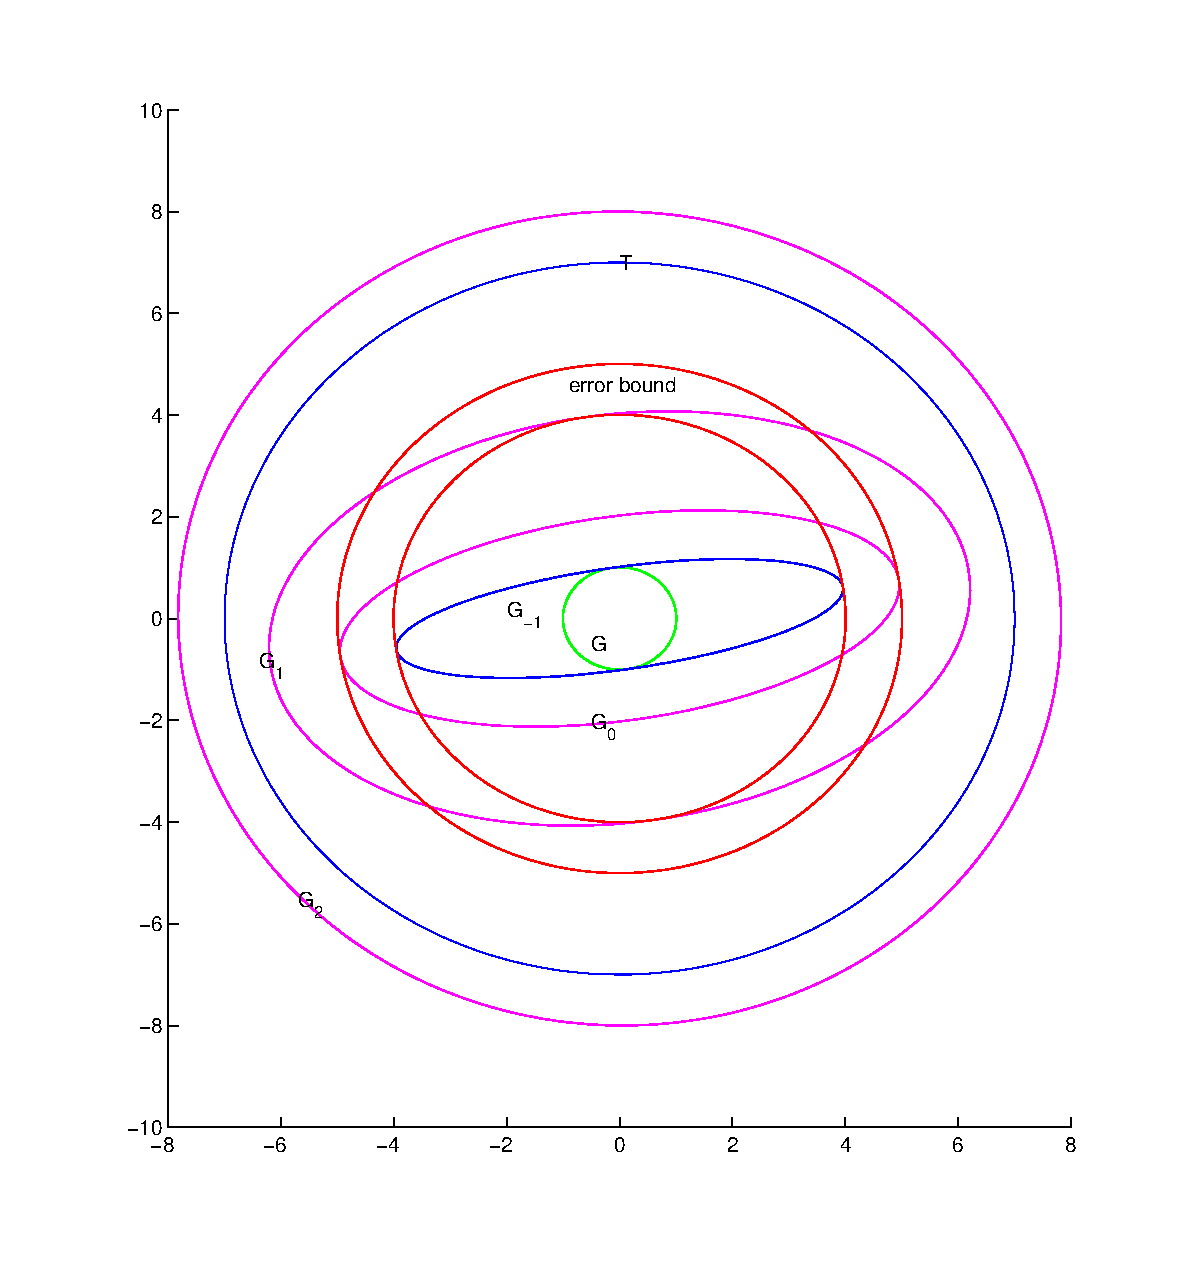
\includegraphics[width = 0.8\textwidth, height = 0.5\textheight]{sys.eps}
%\end{center}
%\caption{Иллюстрация взаимного расположения множеств ошибок в $\mathbb{R}^2$.}
%\label{krasn}
%\end{multicols}
%\end{figure}
\end{remark}

\subsection{Неравенства концентрации для сумм случайных величин ---  неравенства Чернова, Хевдинга, Бернштейна, Азумы}

%По мотивам лекции Голубева, обзора Лугоши.

%\begin{enumerate}
%\item
\begin{problem}[Неравенство  Чернова]

Доказать, что неравенство Чернова для неотрицательной случайной величины $X$
\begin{equation*}
\mathbf{P}\{ X >t\}\leq \inf_{s>0}\mathbf{E}\exp(sX-st)
\end{equation*}
 дает более завышенную границу по сравнению с моментной границей
\begin{equation*}
\mathbf{P}\{ X >t\}\leq \min_{q>0}\mathbf{E}[X^q]t^{-q},
\end{equation*}
 то есть 
\begin{equation*}
\min_q\mathbf{E}[X^q]t^{-q}\leq \inf_{s>0}\mathbf{E}\big[\text{e}^{s(X-t)}\bigl]
\end{equation*}
\end{problem}

\begin{remark} Использовать следствие из неравенства Маркова: для монотонной возрастающей неотрицаиельной функции $\phi(\cdot)$ и произвольной неотрицательной случайной величины $X$ верно
\begin{equation*}
\mathbf{P}\{\phi(X)\geq \phi(t)\}\leq \frac{\mathbf{E}\phi(X)}{\phi(X)}.
\end{equation*}
\end{remark}

%\item 
%\begin{problem}[Неравенство Чернова для суммы случайных величин]

%\end{problem}

%\item
\begin{problem}
Пусть $\xi_t$ ~--- гауссовские случайные величины с нулевым средним и $\mathbf{E}\xi_t^2 = \sigma^2_t\leq\sigma$. Тогда 
\begin{equation*}
\mathbf{E}\max_{t\in T}\xi_t \leq \sqrt{2\sigma^2\log(n)},
\end{equation*}
здесь $n = \#T$~--- число элементов $T$.
\end{problem}
\begin{remark}
Основная идея доказательства: если случайные величины $\xi'_t>0$ имеют тяжелые хвосты, то 
\begin{equation*}
\max_{t\in T} \xi'_t \asymp \sum_{t\in T}\xi'_t.
\end{equation*}

Для любого $\lambda>0$ 
\begin{equation*}
\max_{t\in T} \xi_t = \lambda^{-1}\log\big[\max_{t\in T} \rm e^{\lambda \xi_t}\bigr]\leq \lambda^{-1}\log\big[\sum_{t\in T}\rm e^{\lambda \xi_t}\bigr].
\end{equation*}
Воспользоваться далее неравенством Йенсена и получить
\begin{equation*}
\begin{split}
\mathbf{E}\max_{t\in T} \xi_t \leq \frac{\log(n)}{\lambda} + \frac{\sigma^2\lambda}{2}.
\end{split}
\end{equation*}

Минимизировать по $\lambda$.

\end{remark}
 
\begin{problem}[Лемма Хефдинга] Пусть $X$--- случайная величина, такая что $\mathbf{E}X =0$, $a\leq X\leq b$. Тогда для $s>0$ верно
\begin{equation*}
\mathbf{E}\exp(s X)\leq \exp\bigg[\frac{s^2(b-a)^2}{8}\biggr]
\end{equation*}
\end{problem}

\begin{remark}
Использовать выпуклость экспоненты, для $a\leq x\leq b$

\begin{equation*}
\text{e}^{sx} \leq \frac{x-a}{b-a} \text{e}^{sb}+\frac{b-x}{b-a}\text{e}^{sa} 
\end{equation*}

Получить 

\begin{equation*}
\mathbf{E}\text{e}^{sx} \leq \text{e}^{\phi(u)}
\end{equation*}

где $u = s(b-a)$, $\phi(u) = -pu+\log(1-p+p\text{e}^u)$, $p = -a/(b-a)$.
Найти $\phi^{\prime\prime}(u)$,   $\phi(0)$, $\phi^{\prime}(0)$.

Показать, что 
\begin{equation*}
\phi^{\prime\prime}(u)\leq \frac{1}{4}.
\end{equation*}

Используя формулу Тейлора, получить  
\begin{equation*}
\phi(u) \leq \frac{u^2}{8}\leq \frac{s^2(b-a)^2}{8}.
\end{equation*}
\end{remark}

\begin{problem}[Теорема Хефдинга] Пусть $\xi_t$, $t\in T$ ~--- независимые случайные величины, такие что $\xi_t\in[a,b]$. Тогда
\begin{equation*}
\mathbf{P}\bigg\{\bigg|\frac{1}{n}\sum_{t\in T}\big(\xi_t-\mathbf{E}\xi_t\bigr)\biggr|\geq x\biggr\}\leq 2\exp\bigg\{-\frac{2nx^2}{(b-a)^2}\biggr\}.
\end{equation*}
\end{problem}
\begin{remark}
Ввести случайную величину $\xi = \frac{1}{n}\sum_{i=1}^n(\xi_i-\mathbf{E}\xi_i)$.
Воспользоваться неравеством Чернова и леммой Хевдинга для $\xi$, чтобы получить
\begin{equation*}
\mathbf{P}\{\xi>x\}\leq \exp\bigg\{\min_{\lambda}\bigg[-\lambda x + \frac{\lambda^2}{8}\frac{(b-a)^2}{n}\biggr]\biggr\}.
\end{equation*}
Затем найти оптимальное $\lambda$.  Аналогичное неравенство справедливо для $-\xi$.
\end{remark}

\begin{problem}[Неравенство Беннетта]
Пусть $X_1,\dots, X_n$ независимые центрированные ограниченные случайные величины, такие, что с вероятностью $1$ выполнено $|X_i|\leq c$.
Пусть $\sigma^2 = \sum_{i=1}^n\text{Var}\{X_i\}$.
 Тогда для любого $t>0$ 
\begin{equation*}
\mathbf{P}\bigg\{\sum_{i=1}^n X_i>t\biggr\}\leq \exp\bigg(-\frac{n\sigma^2}{c^2}h\bigg(\frac{ct}{n\sigma^2}\biggr)\biggr),
\end{equation*}
где $h(u) = (1+u)\log(1+u)-u$ для $u\geq 0$.
\end{problem}
\begin{remark}
Введем $\sigma_i^2 = \mathbf{E}[X_i^r]$ и $F_i = \sum_{r=2}^{\infty}\frac{s^{r-2}\mathbf{E}[X_i^r]}{r!\sigma_i^2}$.
Используя разложение для ряда Тейлора $\exp(sX)$, показать, что 
\begin{equation*}
\mathbf{E}[e^{sX_i}]\leq \exp(s^2\sigma^2_iF_i).
\end{equation*}

Из ограниченности  $X_i$ получить оценку
\begin{equation*}
F_i\leq \frac{\exp(sc)-1-sc}{(sc)^2}.
\end{equation*} 
Далее воспользоваться неравенством Чернова для $X_i$ и минимизировать правую часть в неравенстве Чернова по $s$.
\end{remark}

\begin{problem}[Неравенство Бернштейна]
При выполнении условий предыдущей теоремы для любого  $\epsilon>0$ верно 
\begin{equation*}
\mathbf{P}\bigg\{\frac{1}{n}\sum_{i=1}^n X_i>\epsilon\biggr\}\leq \exp\bigg(-\frac{n\epsilon^2}{2\sigma^2+2c\epsilon/3}\biggr).
\end{equation*}
\end{problem}

\begin{remark} 
Показать, что верно элементарное неравенство 
\begin{equation*}
h(u)\geq \frac{u^2}{2+2u/3}
\end{equation*}
и использовать неравенство Беннетта.
\end{remark}
%\end{enumerate}

\begin{problem} Пусть $Y$ случайная величина,  $Y\in [-1,+1]$ и $\mathbf{E}[Y]=0$. Тогда для любого $t\geq 0$ верно 
\begin{equation*}
\mathbf{E}[\exp(tY)]\leq \exp(t^2/2).
\end{equation*}
\end{problem}

\begin{remark}
Использовать выпуклость $\exp(tx)$, а именно для $x\in[-1,1]$ верно.
\begin{equation*}
\text{e}^{tx}\leq \frac{1}{2}(1+x)\text{e}^{t} +\frac{1}{2}(1-x)\text{e}^{-t}
\end{equation*}
Подсчитать оценку математического ожидания $\mathbf{E}[\text{e}^{tY}]$ используя разложение экспоненты в ряд Тейлора и элементарный факт $(2n)!>2^nn!$.  
\end{remark}

\begin{problem}[Мартингальное неравенство Азумы-Хевдинга]

Пусть $\{X_i\}_{i=0}^{\infty}$ мартингал по отношению к фильтрации $\{\mathcal{F}_i\}$, пусть $Y_i = X_i-X_{i-1}$ соответствующая последовательность приращений. Тогда, если существуют такие $c_i>0$, что $|Y_i|\leq c_i$ для всех $i$, то 
\begin{equation*}
\mathbf{P}\{\sup_{n\geq m} |X_n-X_0|\geq t\}\leq 2\exp\bigg\{\frac{-t^2}{2\sum_{i=1}^{m}c^2_i}\biggl\}
\end{equation*}
\end{problem}

\begin{remark}

\begin{enumerate}
\item \textit{Использовать теорему Дуба.} 
%\textbf{TODO}
\item \textit{Cпособ для доказательства не равномерного варианта теоремы использует результат задачи 12.}

Показать, что 
\begin{equation*}
\mathbf{E}\exp(sY_1+\dots+ sY_m) = \mathbf{E}\big[\exp(sY_1+\dots+sY_{m-1})\mathbf{E}[\exp(sY_m)|\mathcal{F}_{m-1}]\bigl] 
\end{equation*}
записать неравенство Чернова

\begin{equation*}
\mathbf{P}[Y_1+\dots+Y_m>t]\leq \exp\big[-st+\sum_{i=1}^mc^2_i s^2/2\bigr].
\end{equation*}
Остается оценить $s$ из минимизации правой части.
\end{enumerate}

\end{remark}



\begin{problem}
Что можно сказать о том, как соотносятся между собой неравенство Бернштейна и Хевдинга? Рассмотреть неравенство Бернштейна в случаях, когда $\sigma^2>\epsilon$ и когда $\sigma^2<\epsilon$. Что можно сказать про достижимость неравенства Бернштейна? 
\begin{remark}
Рассмотреть предельную теорему Пуассона.
\end{remark}
\end{problem}

\subsection{Неравенства концентрации меры для функционалов от случайных величин.}
\medskip

\begin{problem}[Неравенство Эфрона-Стейна]
Пусть $X'_1,\dots,X'_n$ ~--- независимые копии $X_1,\dots,X_n$ и 
\begin{equation*}
Z'_i = g(X_1,\dots, X'_i,\dots,X_n).
\end{equation*}
Тогда верно неравенство 
\begin{equation*}
\text{Var}(Z)\leq \frac{1}{2}\sum_{i=1}^{n}\mathbf{E}[(Z-Z'_i)^2].
\end{equation*}
\end{problem}
\begin{remark}
 
Пусть $X_1,\dots, X_n$, произвольные независимые (не обязательно одинаково распределенные случайные величины) принимающие значения из $\mathcal{X}$ и пусть  $g: \mathcal{X}^n\to \mathbf{R}$ измеримая функция $n$ переменных. Показать, что для случайной величины $Z = g(X_1,\dots,X_n)$ верно 
\begin{equation*}
\text{Var}(Z) \leq \sum_{i=1}^n \mathbf{E}\big[ (Z-\mathbf{E}_iZ)^2\bigl],
\end{equation*}
где $\mathbf{E}_iZ = \mathbf{E}[Z|X_1,\dots,X_{i-1},X_{i+1},\dots,X_n]$.
\end{remark}
\begin{problem}[Случай функций с ограниченными  разностями]
Функция $g: \mathcal{X}^n\to \mathbf{R}$ является функцией с ограниченными разностями, если для некоторых $c_i,$  $1\leq i\leq n$.
\begin{equation*}
\sup_{x_1,\dots,x_n;\, x'_i\in\mathcal{X}} |g(x_1,\dots,x_n)-g(x_1,\dots,x_{i-1},x'_i,x_{i+1},\dots,x_{i+1},\dots,x_n)|\leq c_i. 
\end{equation*}
Выпишите неравенство Эфрона-Стейна для случая функций с ограниченными разностями.
\end{problem}
\medskip

\subsection{Вероятности больших уклонений}


Рассматриваются вероятности $\mathbf{P}\biggl\{\Bigl|\sum_{i=1}^n\xi_i -\sum_{i=1}^m m_i\Bigr|\geq t\biggr\}$ для последовательности независимых величин $\xi_1,\xi_2,\dots$ с математическими ожиданиями $m_i = \mathbf{E} \xi_i$ и $\text{Var} \xi_i = d$. 
Если использовать для оценки этой вероятности неравенство Чебышева, то при $t = c\sqrt{n}$ и $t=cn$, где $c$~--- некоторая постоянная, получается разный порядок сходимости вероятности. В отличае от первого случая, оценка при $t=cn$ является очень грубой. 

\medskip 

Введем ряд обозначений
\begin{equation*}
\mathbf{P}_{n,c} = \mathbf{P}\biggl\{\Bigl|\sum_{i=1}^n\xi_i -\sum_{i=1}^m m_i\Bigr|\geq cn\biggr\},
\end{equation*}
\begin{equation*}
R(\lambda)=\int_{-\infty}^{\infty}\text{e}^{\lambda x}\,d F(x),
\end{equation*}
\begin{equation*}
m(\lambda) = \frac{R^{\prime}(\lambda)}{R(\lambda)}.
\end{equation*}

\medskip

Оказывается, что при условии 
\begin{equation}
R(\lambda)<\infty
\label{condition.R}
\end{equation}
верна более точная оценка 
\begin{equation*}
\lim_{n\to\infty}\frac{1}{n}\ln \mathbf{P}_{n,c} =\ln r(\lambda_0),
\end{equation*}
где 
\begin{equation*}
r(\lambda_0) = \text{e}^{-\lambda_0 c}R(\lambda_0),
\end{equation*}
значение $\lambda_0$ удовлетворяет условию  $m(\lambda_0) = c$.

\medskip

Для того, чтобы это показать, докажите следующие утверждения.

\begin{problem}
Будем говорить, что $M^{+}$ есть верхний предел по вероятности случайной величины $\xi$, если $\mathbf{P}\{\xi>M^{+}\} = 0$ и $\mathbf{P}\{M^{+}-\epsilon\leq\xi\leq M^{+}\}>0$ для каждого  $\epsilon>0$. Нижний предел по вероятности можно определить тем же образом. Если $\mathbf{P}\{\xi>M\}>0$, ($\mathbf{P}\{\xi<M\}>0$) для всякого $M$, то $M^{+}=\infty$ ($M^{-}=-\infty$). Во всех остальных случаях $M^{+}$ и $M^{-}$ конечны.
Показать, что при условии \eqref{condition.R} 
функция $m(\lambda)$ имеет следующие пределы
\begin{equation*}
\lim_{\lambda\to\infty}m(\lambda) = M^{+},\quad \lim_{\lambda\to -\infty} = M^{-}.
\end{equation*}
\end{problem}
%\begin{remark}

%\textbf{TODO}

%\end{remark}
\begin{problem}
Имеет место неравенство 
\begin{equation*}
\mathbf{P}_{n,c} \leq B_n(R(\lambda_0)\text{e}^{-\lambda_0c})^n,\quad\text{где} \lim_{n\to\infty}B_n=\frac{1}{2}.
\end{equation*}
\end{problem}
%\begin{remark}

%\textbf{TODO}

%\end{remark}
\begin{problem}
Для всякого $b>0$ существует такое $p(b,\lambda_0)>0$, что 
\begin{equation*}
\mathbf{P}_{n,c} \geq (R(\lambda_0)\text{e}^{-\lambda_0c})^n\text{e}^{-\lambda_0 b \sqrt{n}} p_n, 
\end{equation*}
причем $\lim_{n\to\infty}p_n = p(b,\lambda_0)$.
\end{problem}
%\begin{remark}
%\textbf{TODO}
%\end{remark}
%\begin{problem}[Задача о среднем функции в смысле Леви --- про концентрацию меры на сфере вокруг медианного значения "хорошей" функции]
%\end{problem}
%\subsection{Изопериметрические неравенства Талаграна(?)}
